%%%%%%%%%%%%%%%%%%%%%%%%%%%%%%%%%%%%%%%%%
% Programming/Coding Assignment
% LaTeX Template
%
% This template has been downloaded from:
% http://www.latextemplates.com
%
% Original author:
% Ted Pavlic (http://www.tedpavlic.com)
%
% Note:
% The \lipsum[#] commands throughout this template generate dummy text
% to fill the template out. These commands should all be removed when 
% writing assignment content.
%
% This template uses a Perl script as an example snippet of code, most other
% languages are also usable. Configure them in the "CODE INCLUSION 
% CONFIGURATION" section.
%
%%%%%%%%%%%%%%%%%%%%%%%%%%%%%%%%%%%%%%%%%

%----------------------------------------------------------------------------------------
%	PACKAGES AND OTHER DOCUMENT CONFIGURATIONS
%----------------------------------------------------------------------------------------

\documentclass{article}

\usepackage{fancyhdr} % Required for custom headers
\usepackage{lastpage} % Required to determine the last page for the footer
\usepackage{extramarks} % Required for headers and footers
\usepackage[usenames,dvipsnames]{color} % Required for custom colors
\usepackage{graphicx} % Required to insert images
\usepackage{subcaption}
\usepackage{listings} % Required for insertion of code
\usepackage{courier} % Required for the courier font


% Margins
\topmargin=-0.45in
\evensidemargin=0in
\oddsidemargin=0in
\textwidth=6.5in
\textheight=9.0in
\headsep=0.25in

\linespread{1.1} % Line spacing

% Set up the header and footer
\pagestyle{fancy}
\lhead{\hmwkAuthorName} % Top left header
\chead{\hmwkClass\ (\hmwkClassTime): \hmwkTitle} % Top center head
%\rhead{\firstxmark} % Top right header
\lfoot{\lastxmark} % Bottom left footer
\cfoot{} % Bottom center footer
\rfoot{Page\ \thepage\ of\ \protect\pageref{LastPage}} % Bottom right footer
\renewcommand\headrulewidth{0.4pt} % Size of the header rule
\renewcommand\footrulewidth{0.4pt} % Size of the footer rule

\setlength\parindent{0pt} % Removes all indentation from paragraphs

%----------------------------------------------------------------------------------------
%	CODE INCLUSION CONFIGURATION
%----------------------------------------------------------------------------------------

\definecolor{MyDarkGreen}{rgb}{0.0,0.4,0.0} % This is the color used for comments
\lstloadlanguages{Perl} % Load Perl syntax for listings, for a list of other languages supported see: ftp://ftp.tex.ac.uk/tex-archive/macros/latex/contrib/listings/listings.pdf
\lstset{language=Perl, % Use Perl in this example
        frame=single, % Single frame around code
        basicstyle=\small\ttfamily, % Use small true type font
        keywordstyle=[1]\color{Blue}\bf, % Perl functions bold and blue
        keywordstyle=[2]\color{Purple}, % Perl function arguments purple
        keywordstyle=[3]\color{Blue}\underbar, % Custom functions underlined and blue
        identifierstyle=, % Nothing special about identifiers                                         
        commentstyle=\usefont{T1}{pcr}{m}{sl}\color{MyDarkGreen}\small, % Comments small dark green courier font
        stringstyle=\color{Purple}, % Strings are purple
        showstringspaces=false, % Don't put marks in string spaces
        tabsize=5, % 5 spaces per tab
        %
        % Put standard Perl functions not included in the default language here
        morekeywords={rand},
        %
        % Put Perl function parameters here
        morekeywords=[2]{on, off, interp},
        %
        % Put user defined functions here
        morekeywords=[3]{test},
       	%
        morecomment=[l][\color{Blue}]{...}, % Line continuation (...) like blue comment
        numbers=left, % Line numbers on left
        firstnumber=1, % Line numbers start with line 1
        numberstyle=\tiny\color{Blue}, % Line numbers are blue and small
        stepnumber=5 % Line numbers go in steps of 5
}

% Creates a new command to include a perl script, the first parameter is the filename of the script (without .pl), the second parameter is the caption
\newcommand{\perlscript}[2]{
\begin{itemize}
\item[]\lstinputlisting[caption=#2,label=#1]{#1.pl}
\end{itemize}
}

%----------------------------------------------------------------------------------------
%	DOCUMENT STRUCTURE COMMANDS
%	Skip this unless you know what you're doing
%----------------------------------------------------------------------------------------

% Header and footer for when a page split occurs within a problem environment
\newcommand{\enterProblemHeader}[1]{
%\nobreak\extramarks{#1}{#1 continued on next page\ldots}\nobreak
%\nobreak\extramarks{#1 (continued)}{#1 continued on next page\ldots}\nobreak
}

% Header and footer for when a page split occurs between problem environments
\newcommand{\exitProblemHeader}[1]{
%\nobreak\extramarks{#1 (continued)}{#1 continued on next page\ldots}\nobreak
%\nobreak\extramarks{#1}{}\nobreak
}

\setcounter{secnumdepth}{0} % Removes default section numbers
\newcounter{homeworkProblemCounter} % Creates a counter to keep track of the number of problems
\setcounter{homeworkProblemCounter}{0}

\newcommand{\homeworkProblemName}{}
\newenvironment{homeworkProblem}[1][Problem \arabic{homeworkProblemCounter}]{ % Makes a new environment called homeworkProblem which takes 1 argument (custom name) but the default is "Problem #"
\stepcounter{homeworkProblemCounter} % Increase counter for number of problems
\renewcommand{\homeworkProblemName}{#1} % Assign \homeworkProblemName the name of the problem
\section{\homeworkProblemName} % Make a section in the document with the custom problem count
\enterProblemHeader{\homeworkProblemName} % Header and footer within the environment
}{
\exitProblemHeader{\homeworkProblemName} % Header and footer after the environment
}

\newcommand{\problemAnswer}[1]{ % Defines the problem answer command with the content as the only argument
\noindent\framebox[\columnwidth][c]{\begin{minipage}{0.98\columnwidth}#1\end{minipage}} % Makes the box around the problem answer and puts the content inside
}

\newcommand{\homeworkSectionName}{}
\newenvironment{homeworkSection}[1]{ % New environment for sections within homework problems, takes 1 argument - the name of the section
\renewcommand{\homeworkSectionName}{#1} % Assign \homeworkSectionName to the name of the section from the environment argument
\subsection{\homeworkSectionName} % Make a subsection with the custom name of the subsection
\enterProblemHeader{\homeworkProblemName\ [\homeworkSectionName]} % Header and footer within the environment
}{
\enterProblemHeader{\homeworkProblemName} % Header and footer after the environment
}

%----------------------------------------------------------------------------------------
%	NAME AND CLASS SECTION
%----------------------------------------------------------------------------------------

\newcommand{\hmwkTitle}{Project\ \#1} % Assignment title
\newcommand{\hmwkDueDate}{Monday,\ January\ 29,\ 2018} % Due date
\newcommand{\hmwkClass}{CSC411} % Course/class
\newcommand{\hmwkClassTime}{L0501} % Class/lecture time
\newcommand{\hmwkAuthorName}{Xiangyu Kong} % Your name

%----------------------------------------------------------------------------------------
%	TITLE PAGE
%----------------------------------------------------------------------------------------

\title{
\vspace{2in}
\textmd{\textbf{\hmwkClass:\ \hmwkTitle}}\\
\normalsize\vspace{0.1in}\small{Due\ on\ \hmwkDueDate}\\
\vspace{0.1in}
\vspace{3in}
}

\author{\textbf{\hmwkAuthorName}}
\date{} % Insert date here if you want it to appear below your name

%----------------------------------------------------------------------------------------

\begin{document}

\maketitle
\clearpage
%----------------------------------------------------------------------------------------
%	PROBLEM 1
%----------------------------------------------------------------------------------------

% To have just one problem per page, simply put a \clearpage after each problem

\begin{homeworkProblem}

\noindent \textit{Dataset description}

The dataset consists of $1691$ gray-scale $32 \times 32$-pixel of images of $12$ different actor/actress's faces. The angle, lighting and expressions for the faces are all different (as shown in Figure~\ref{fig:uncropped1} and Figure~\ref{fig:uncropped2}). Some faces aren't fully shown (as shown in Figure~\ref{fig:uncropped3}). After cropping their faces out, examining the dataset, most of the faces are correctly cropped given the coordinates (Figure~\ref{fig:cropped1}), but there are still incorrect coordinates that leads to incorrect faces (Figure~\ref{fig:cropped2}). Also, some cropped faces are not aligned together. e.g. Some are center aligned and some are not (Figure~\ref{fig:cropped1} and Figure~\ref{fig:cropped3}).

\begin{figure*}[!ht]
	\begin{subfigure}{.35\textwidth}
		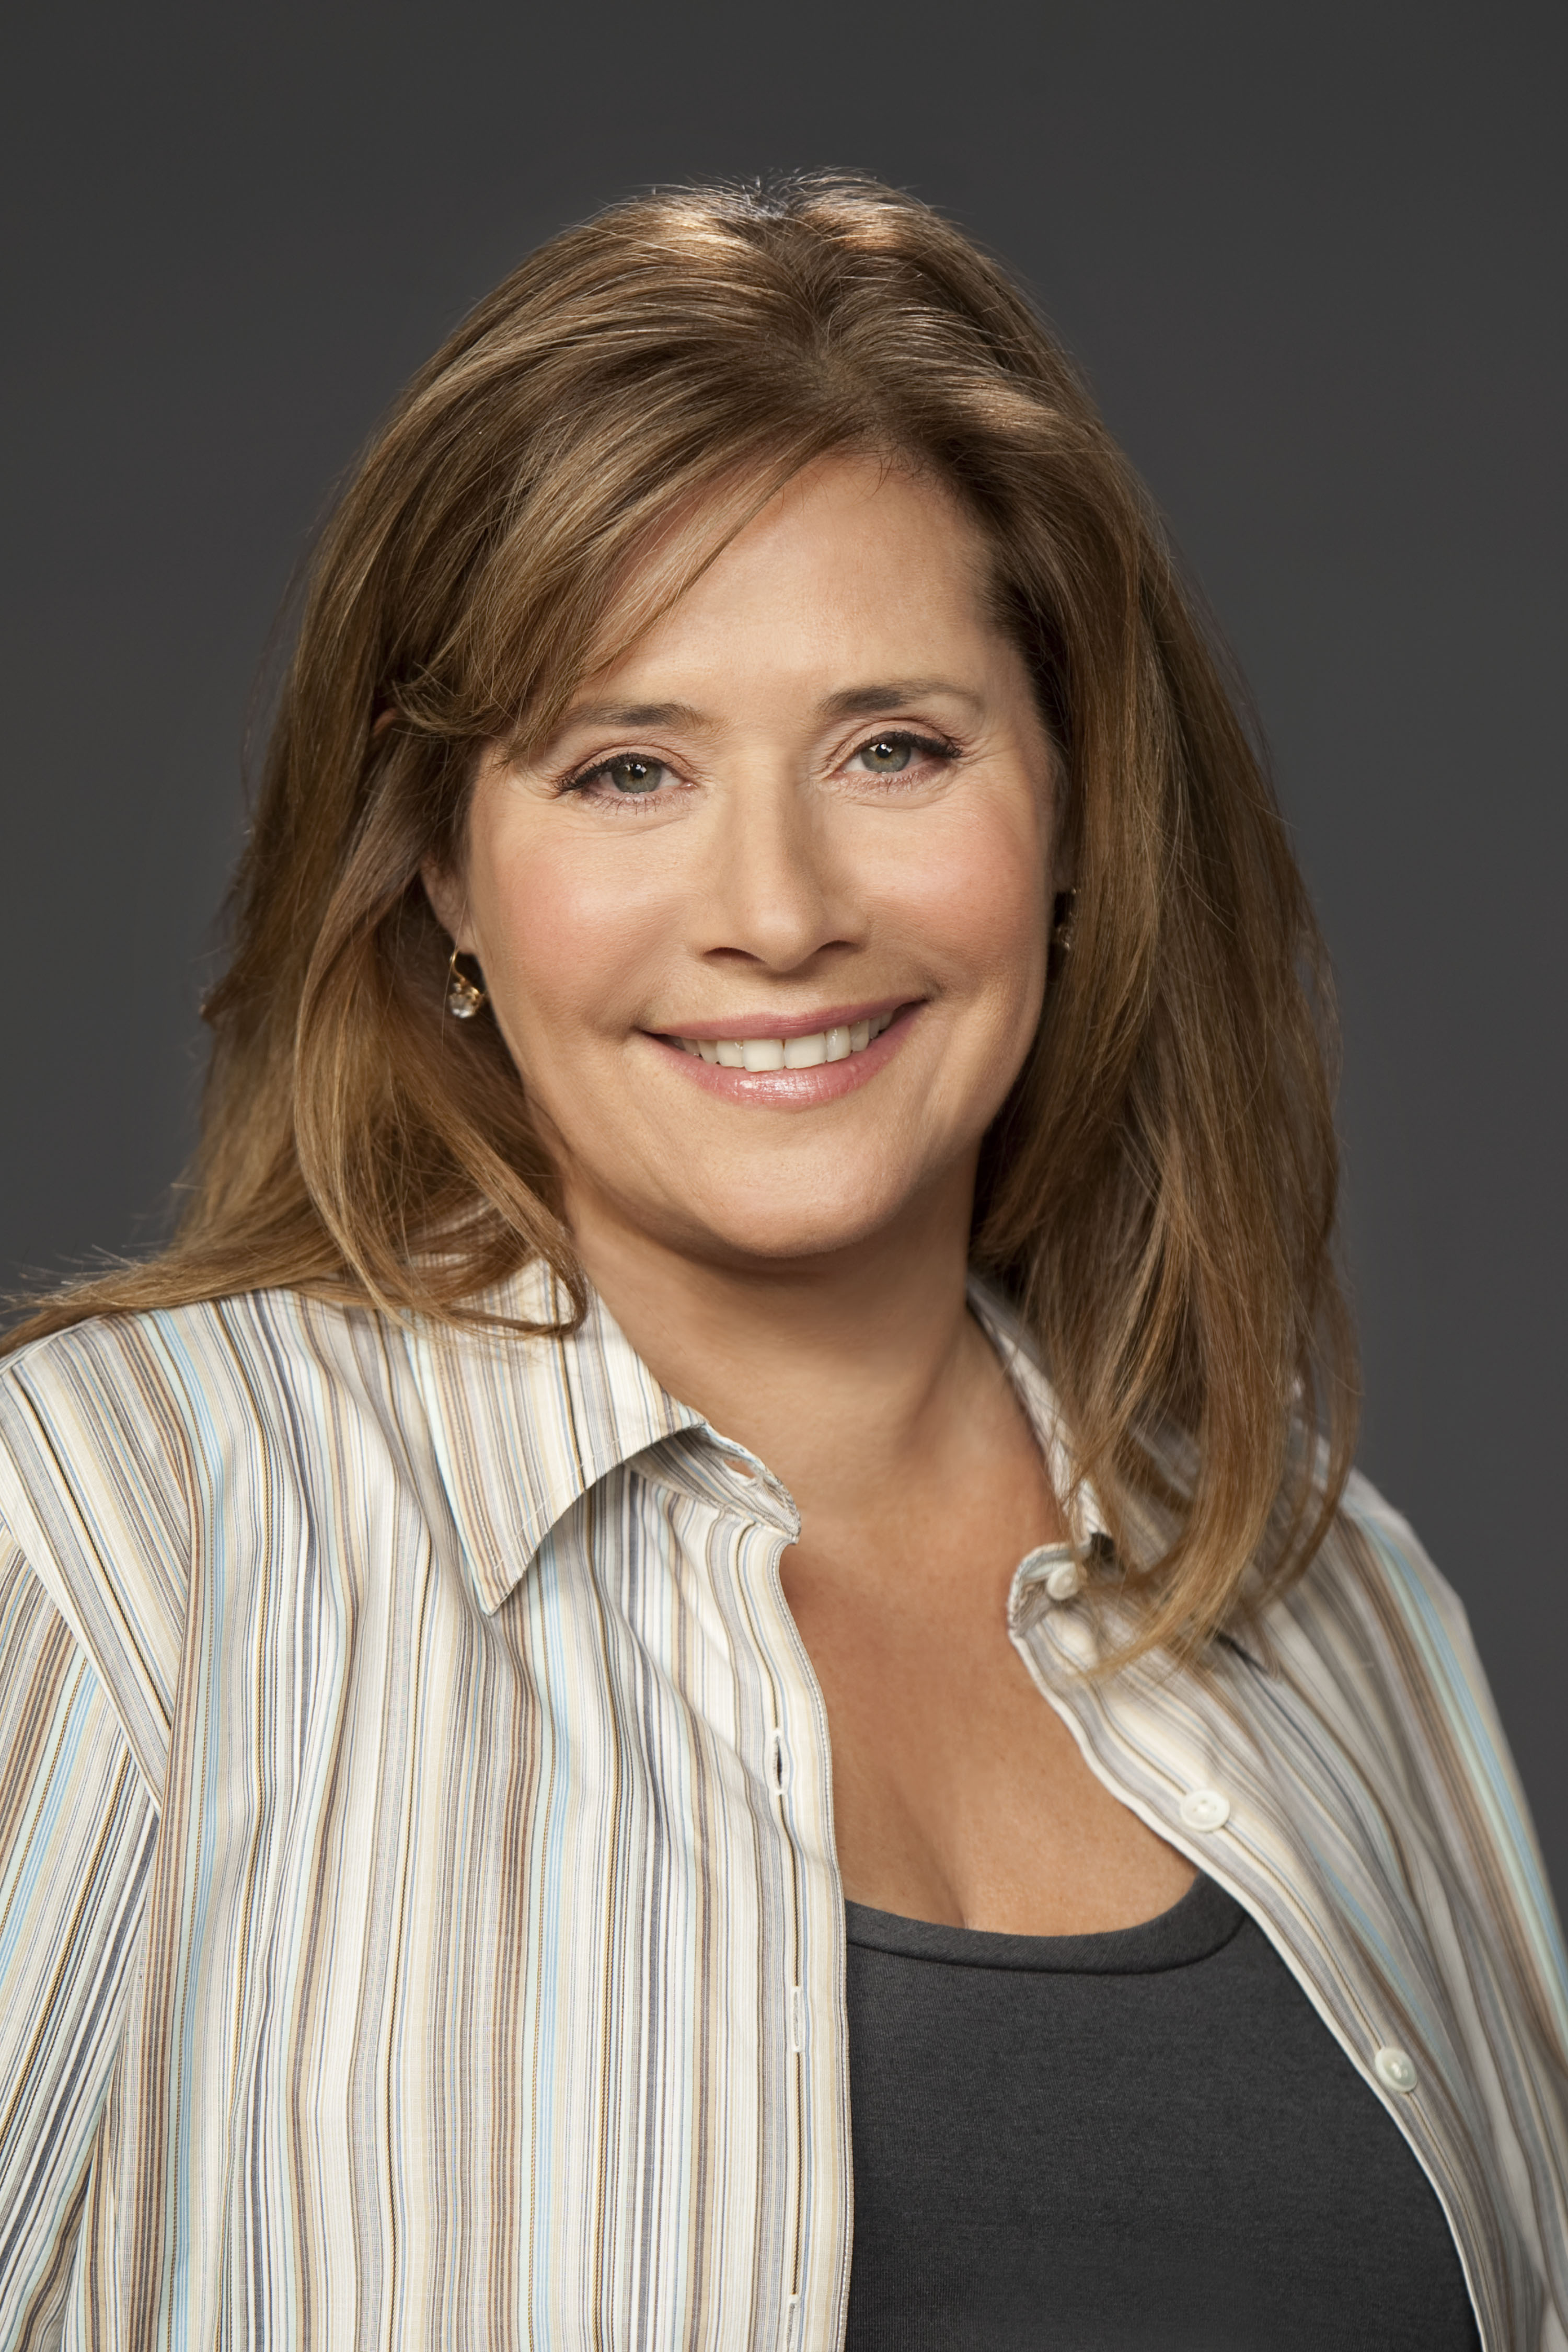
\includegraphics[width=.35\linewidth]{images/1/1.jpg}
		\caption{front}
		\label{fig:uncropped1}
	\end{subfigure}
	\begin{subfigure}{.35\textwidth}
		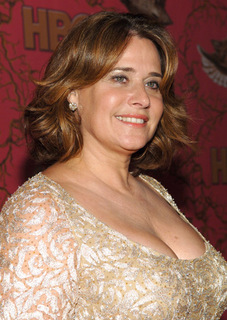
\includegraphics[width=.35\linewidth]{images/1/2.jpg}
		\caption{side}
		\label{fig:uncropped2}
	\end{subfigure}%
	\begin{subfigure}{.35\textwidth}
		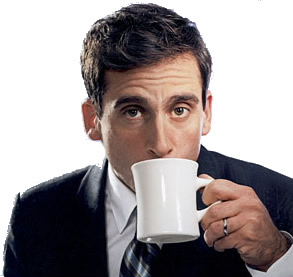
\includegraphics[width=.35\linewidth]{images/1/3.jpg}
		\caption{blocked face}
		\label{fig:uncropped3}
	\end{subfigure}
	\begin{subfigure}{.35\textwidth}
		
\includegraphics[width=.35\linewidth]{images/1/4.jpg}
		\caption{correctly cropped}
		\label{fig:cropped1}
	\end{subfigure}%
	\begin{subfigure}{.35\textwidth}
		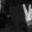
\includegraphics[width=.35\linewidth]{images/1/5.jpg}
		\caption{incorrect coordinates for face}
		\label{fig:cropped2}
	\end{subfigure}
	\begin{subfigure}{.35\textwidth}
		
\includegraphics[width=.35\linewidth]{images/1/6.jpg}
		\caption{face not aligned to the center}
		\label{fig:cropped3}
	\end{subfigure}
	\caption{}
	\label{fig:pcs}
\end{figure*}

\end{homeworkProblem}
\clearpage

%%----------------------------------------------------------------------------------------
%%	PROBLEM 2
%%----------------------------------------------------------------------------------------

\begin{homeworkProblem}
\noindent \textit{Separating the sets.}

The algorithm for separating the sets of data is to first shuffle the data as a list, then through list slicing, first pick $10$ images as the test set, then pick $10$ images as the validation set, and finally the rest are used as the training set.


\end{homeworkProblem}
\clearpage

%----------------------------------------------------------------------------------------
%	PROBLEM 3
%----------------------------------------------------------------------------------------

\begin{homeworkProblem}
\noindent \textit{Linear classifier to distinguish between Alec Baldwin from Steve Carell}

Using the divided data sets from part 2, the program trains the linear classifier by gradient descent and then apply the classifier to the validation set and the test set.\\

The functions to compute the output are as follows (all print statements are removed for simplicity):\\
\begin{lstlisting}[language=Python, caption=Gradient Descent]
def grad_descent(loss, dlossdx, x, y, init_theta, alpha):
	eps = 1e-5
	prev_theta = init_theta - 10 * eps
	theta = init_theta.copy()
	max_iter = 100000
	i = 0	
	while norm(theta - prev_theta) > eps and i < max_iter:
		prev_theta = theta.copy()
		theta -= alpha * dlossdx(x, y, theta)
		i += 1
	return theta
\end{lstlisting}

\begin{lstlisting}[language=Python, caption=Predict]
def predict(im, theta):
	data = imread("./cropped/" + im) / 225.
	data = reshape(data, 1024)
	data = np.insert(data, 0, 1)
	prediction = np.dot(data, theta)
	return prediction
\end{lstlisting}

\begin{lstlisting}[language=Python, caption=Test]
theta = grad_descent(loss, dlossdx, x, y, theta, 0.005)
for im in validation_set:
	prediction = predict(im, theta)
	if im in actor1_validation_set and norm(prediction) > 0.5:
		correct_count += 1
	elif im in actor2_validation_set and norm(prediction) <= 0.5:
		correct_count += 1
\end{lstlisting}

In order for the system to work, I had to keep track of each vector/matrix's shape and when to use their transpose in order for the multiplication to work. Also, I had to tune the alpha value and the iteration value. This is because if the alpha value is too small, the gradient descent will be too slow so more iterations are required, and if the alpha value is too large, numpy will give $nan$ on the trained gradients.

\end{homeworkProblem}
\clearpage

%%----------------------------------------------------------------------------------------
%%	PROBLEM 4
%%----------------------------------------------------------------------------------------
%
%\begin{homeworkProblem}
%\noindent \textit{Reconstructing images where salt-and-pepper noise was applied}
%
%Noisy images are created using the function \texttt{salt\_and\_pepper\_noise()} (lines 98-106 of \texttt{pca\_example.py}). \\
%The function \texttt{salt\_and\_pepper\_noise()} randomly sets a subselection of pixels to 0 or 1, while $noise\_prop$ is the proportion of the pixels set to either 0 or 1.
%Once the salt-and-pepper noise is applied, the images are reconstructed using 200 principal components using the function 
%\texttt{get\_reconstruction()} (lines 65-70 and 167-317 of \texttt{pca\_example.py}). 
%
%We vary the proportion of pixels that are perturbed using salt-and-pepper-noise.
%
%Some results are shown in  Figure~\ref{fig:a0all}, Figure~\ref{fig:a2all}, Figure~\ref{fig:a10all}, Figure~\ref{fig:a15all}.
%
%For moderate amounts of noise, we are able to get a reconstruction that looks similar to the original image, without the noise.
%
%After the proportion of pixels that are perturbed becomes greater than a certain threshold, (the threshold varies from one letter to another), the reconstruction gets worse and worse and eventually stops producing an image that looks like an 'a'.
%The threshold in Figure~\ref{fig:a0all} and in Figure~\ref{fig:a10all} is around 60\% ($noise\_prop = 0.6$). 
%That of Figure~\ref{fig:a2all} is around 45\% ($noise\_prop = 0.45$). 
%Figure~\ref{fig:a15all} has the lowest threshold out of these four examples, at around 20\% ($noise\_prop = 0.2$).
%
%\textit{Advice: look at the results, point out where the algorithm works, and where the algorithm doesn't work.}
%
%\begin{figure*}[!ht]
%\begin{subfigure}{.35\textwidth}
%  \centering
%  \includegraphics[width=.35\linewidth]{a0reconstruction.jpg}
%  \caption{Original image}
%  \label{fig:a0}
%\end{subfigure}%
%
%\begin{subfigure}{.35\textwidth}
%  \centering
%  \includegraphics[width=.35\linewidth]{a0noise0pt05.jpg}
%  \caption{Image~\ref{fig:a0} with 5\% noise}
%  \label{fig:a0noise0.05}
%\end{subfigure}%
%\begin{subfigure}{.35\textwidth}
%  \centering
%  \includegraphics[width=.35\linewidth]{a0noise0pt05reconstruction200PCs.jpg}
%  \caption{Reconstruction of Image~\ref{fig:a0noise0.05} using 200 principal components}
%  \label{fig:a0noise0.05reconstruction}
%\end{subfigure}%
%
%\begin{subfigure}{.35\textwidth}
%  \centering
%  \includegraphics[width=.35\linewidth]{a0noise0pt1.jpg}
%  \caption{Image~\ref{fig:a0} with 10\% noise}
%  \label{fig:a0noise0.1}
%\end{subfigure}%
%\begin{subfigure}{.35\textwidth}
%  \centering
%  \includegraphics[width=.35\linewidth]{a0noise0pt1reconstruction200PCs.jpg}
%  \caption{Reconstruction of Image~\ref{fig:a0noise0.1} using 200 principal components}
%  \label{fig:a0noise0.1reconstruction}
%\end{subfigure}%
%
%\begin{subfigure}{.35\textwidth}
%  \centering
%  \includegraphics[width=.35\linewidth]{a0noise0pt2.jpg}
%  \caption{Image~\ref{fig:a0} with 20\% noise}
%  \label{fig:a0noise0.2}
%\end{subfigure}%
%\begin{subfigure}{.35\textwidth}
%  \centering
%  \includegraphics[width=.35\linewidth]{a0noise0pt2reconstruction200PCs.jpg}
%  \caption{Reconstruction of Image~\ref{fig:a0noise0.2} using 200 principal components}
%  \label{fig:a0noise0.2reconstruction}
%\end{subfigure}%
%
%\begin{subfigure}{.35\textwidth}
%  \centering
%  \includegraphics[width=.35\linewidth]{a0noise0pt3.jpg}
%  \caption{Image~\ref{fig:a0} with 30\% noise}
%  \label{fig:a0noise0.3}
%\end{subfigure}%
%\begin{subfigure}{.35\textwidth}
%  \centering
%  \includegraphics[width=.35\linewidth]{a0noise0pt3reconstruction200PCs.jpg}
%  \caption{Reconstruction of Image~\ref{fig:a0noise0.3} using 200 principal components}
%  \label{fig:a0noise0.3reconstruction}
%\end{subfigure}%
%
%\begin{subfigure}{.35\textwidth}
%  \centering
%  \includegraphics[width=.35\linewidth]{a0noise0pt45.jpg}
%  \caption{Image~\ref{fig:a0} with 45\% noise}
%  \label{fig:a0noise0.45}
%\end{subfigure}%
%\begin{subfigure}{.35\textwidth}
%  \centering
%  \includegraphics[width=.35\linewidth]{a0noise0pt45reconstruction200PCs.jpg}
%  \caption{Reconstruction of Image~\ref{fig:a0noise0.45} using 200 principal components}
%  \label{fig:a0noise0.45reconstruction}
%\end{subfigure}%
%
%\begin{subfigure}{.35\textwidth}
%  \centering
%  \includegraphics[width=.35\linewidth]{a0noise0pt60.jpg}
%  \caption{Image~\ref{fig:a0} with 60\% noise}
%  \label{fig:a0noise0.60}
%\end{subfigure}%
%\begin{subfigure}{.35\textwidth}
%  \centering
%  \includegraphics[width=.35\linewidth]{a0noise0pt60reconstruction200PCs.jpg}
%  \caption{Reconstruction of Image~\ref{fig:a0noise0.60} using 200 principal components}
%  \label{fig:a0noise0.60reconstruction}
%\end{subfigure}%
%
%\caption{}
%\label{fig:a0all}
%\end{figure*}
%
%%%%%%%%%%%%%%%%%%%%%%%%%%%%%%%%%%%%%%%%%%%%%%%%%%%%%%%%%%%%%%%%%%%%%%%%
%
%\begin{figure*}[!ht]
%\begin{subfigure}{.35\textwidth}
%  \centering
%  \includegraphics[width=.35\linewidth]{a2reconstruction.jpg}
%  \caption{Original image}
%  \label{fig:a2}
%\end{subfigure}%15
%
%\begin{subfigure}{.35\textwidth}
%  \centering
%  \includegraphics[width=.35\linewidth]{a2noise0pt05.jpg}
%  \caption{Image~\ref{fig:a2} with 5\% noise}
%  \label{fig:a2noise0.05}
%\end{subfigure}%
%\begin{subfigure}{.35\textwidth}
%  \centering
%  \includegraphics[width=.35\linewidth]{a2noise0pt05reconstruction200PCs.jpg}
%  \caption{Reconstruction of Image~\ref{fig:a2noise0.05} using 200 principal components}
%  \label{fig:a2noise0.05reconstruction}
%\end{subfigure}%
%
%\begin{subfigure}{.35\textwidth}
%  \centering
%  \includegraphics[width=.35\linewidth]{a2noise0pt1.jpg}
%  \caption{Image~\ref{fig:a2} with 10\% noise}
%  \label{fig:a2noise0.1}
%\end{subfigure}%
%\begin{subfigure}{.35\textwidth}
%  \centering
%  \includegraphics[width=.35\linewidth]{a2noise0pt1reconstruction200PCs.jpg}
%  \caption{Reconstruction of Image~\ref{fig:a2noise0.1} using 200 principal components}
%  \label{fig:a2noise0.1reconstruction}
%\end{subfigure}%
%
%\begin{subfigure}{.35\textwidth}
%  \centering
%  \includegraphics[width=.35\linewidth]{a2noise0pt2.jpg}
%  \caption{Image~\ref{fig:a2} with 20\% noise}
%  \label{fig:a2noise0.2}
%\end{subfigure}%
%\begin{subfigure}{.35\textwidth}
%  \centering
%  \includegraphics[width=.35\linewidth]{a2noise0pt2reconstruction200PCs.jpg}
%  \caption{Reconstruction of Image~\ref{fig:a2noise0.2} using 200 principal components}
%  \label{fig:a2noise0.2reconstruction}
%\end{subfigure}%
%
%\begin{subfigure}{.35\textwidth}
%  \centering
%  \includegraphics[width=.35\linewidth]{a2noise0pt3.jpg}
%  \caption{Image~\ref{fig:a2} with 30\% noise}
%  \label{fig:a2noise0.3}
%\end{subfigure}%
%\begin{subfigure}{.35\textwidth}
%  \centering
%  \includegraphics[width=.35\linewidth]{a2noise0pt3reconstruction200PCs.jpg}
%  \caption{Reconstruction of Image~\ref{fig:a2noise0.3} using 200 principal components}
%  \label{fig:a2noise0.3reconstruction}
%\end{subfigure}%
%
%\begin{subfigure}{.35\textwidth}
%  \centering
%  \includegraphics[width=.35\linewidth]{a2noise0pt45.jpg}
%  \caption{Image~\ref{fig:a2} with 45\% noise}
%  \label{fig:a2noise0.45}
%\end{subfigure}%
%\begin{subfigure}{.35\textwidth}
%  \centering
%  \includegraphics[width=.35\linewidth]{a2noise0pt45reconstruction200PCs.jpg}
%  \caption{Reconstruction of Image~\ref{fig:a2noise0.45} using 200 principal components}
%  \label{fig:a2noise0.45reconstruction}
%\end{subfigure}%
%
%\begin{subfigure}{.35\textwidth}
%  \centering
%  \includegraphics[width=.35\linewidth]{a2noise0pt60.jpg}
%  \caption{Image~\ref{fig:a2} with 60\% noise}
%  \label{fig:a2noise0.60}
%\end{subfigure}%
%\begin{subfigure}{.35\textwidth}
%  \centering
%  \includegraphics[width=.35\linewidth]{a2noise0pt60reconstruction200PCs.jpg}
%  \caption{Reconstruction of Image~\ref{fig:a2noise0.60} using 200 principal components}
%  \label{fig:a2noise0.60reconstruction}
%\end{subfigure}%
%
%\caption{}
%\label{fig:a2all}
%\end{figure*}
%
%\begin{figure*}[!ht]
%\begin{subfigure}{.35\textwidth}
%  \centering
%  \includegraphics[width=.35\linewidth]{a10reconstruction.jpg}
%  \caption{Original image}
%  \label{fig:a10}
%\end{subfigure}%
%
%\begin{subfigure}{.35\textwidth}
%  \centering
%  \includegraphics[width=.35\linewidth]{a10noise0pt05.jpg}
%  \caption{Image~\ref{fig:a10} with 5\% noise}
%  \label{fig:a10noise0.05}
%\end{subfigure}%
%\begin{subfigure}{.35\textwidth}
%  \centering
%  \includegraphics[width=.35\linewidth]{a10noise0pt05reconstruction200PCs.jpg}
%  \caption{Reconstruction of Image~\ref{fig:a10noise0.05} using 200 principal components}
%  \label{fig:a10noise0.05reconstruction}
%\end{subfigure}%
%
%\begin{subfigure}{.35\textwidth}
%  \centering
%  \includegraphics[width=.35\linewidth]{a10noise0pt1.jpg}
%  \caption{Image~\ref{fig:a10} with 10\% noise}
%  \label{fig:a10noise0.1}
%\end{subfigure}%
%\begin{subfigure}{.35\textwidth}
%  \centering
%  \includegraphics[width=.35\linewidth]{a10noise0pt1reconstruction200PCs.jpg}
%  \caption{Reconstruction of Image~\ref{fig:a10noise0.1} using 200 principal components}
%  \label{fig:a10noise0.1reconstruction}
%\end{subfigure}%
%
%\begin{subfigure}{.35\textwidth}
%  \centering
%  \includegraphics[width=.35\linewidth]{a10noise0pt2.jpg}
%  \caption{Image~\ref{fig:a10} with 20\% noise}
%  \label{fig:a10noise0.2}
%\end{subfigure}%
%\begin{subfigure}{.35\textwidth}
%  \centering
%  \includegraphics[width=.35\linewidth]{a10noise0pt2reconstruction200PCs.jpg}
%  \caption{Reconstruction of Image~\ref{fig:a10noise0.2} using 200 principal components}
%  \label{fig:a10noise0.2reconstruction}
%\end{subfigure}%
%
%\begin{subfigure}{.35\textwidth}
%  \centering
%  \includegraphics[width=.35\linewidth]{a10noise0pt3.jpg}
%  \caption{Image~\ref{fig:a10} with 30\% noise}
%  \label{fig:a10noise0.3}
%\end{subfigure}%
%\begin{subfigure}{.35\textwidth}
%  \centering
%  \includegraphics[width=.35\linewidth]{a10noise0pt3reconstruction200PCs.jpg}
%  \caption{Reconstruction of Image~\ref{fig:a10noise0.3} using 200 principal components}
%  \label{fig:a10noise0.3reconstruction}
%\end{subfigure}%
%
%\begin{subfigure}{.35\textwidth}
%  \centering
%  \includegraphics[width=.35\linewidth]{a10noise0pt45.jpg}
%  \caption{Image~\ref{fig:a10} with 45\% noise}
%  \label{fig:a10noise0.45}
%\end{subfigure}%
%\begin{subfigure}{.35\textwidth}
%  \centering
%  \includegraphics[width=.35\linewidth]{a10noise0pt45reconstruction200PCs.jpg}
%  \caption{Reconstruction of Image~\ref{fig:a10noise0.45} using 200 principal components}
%  \label{fig:a10noise0.45reconstruction}
%\end{subfigure}%
%
%\begin{subfigure}{.35\textwidth}
%  \centering
%  \includegraphics[width=.35\linewidth]{a10noise0pt60.jpg}
%  \caption{Image~\ref{fig:a10} with 60\% noise}
%  \label{fig:a10noise0.60}
%\end{subfigure}%
%\begin{subfigure}{.35\textwidth}
%  \centering
%  \includegraphics[width=.35\linewidth]{a10noise0pt60reconstruction200PCs.jpg}
%  \caption{Reconstruction of Image~\ref{fig:a10noise0.60} using 200 principal components}
%  \label{fig:a10noise0.60reconstruction}
%\end{subfigure}%
%
%\caption{}
%\label{fig:a10all}
%\end{figure*}
%%%%%%%%%%%%%%%%%%%%%%%%%%%%%%%%%%%%%%%%%%%%%%%%%%%%%%%%%%%%%%%%%%%%%%%%
%\begin{figure*}[!ht]
%\begin{subfigure}{.35\textwidth}
%  \centering
%  \includegraphics[width=.35\linewidth]{a15reconstruction.jpg}
%  \caption{Original image}
%  \label{fig:a15}
%\end{subfigure}%15
%
%\begin{subfigure}{.35\textwidth}
%  \centering
%  \includegraphics[width=.35\linewidth]{a15noise0pt05.jpg}
%  \caption{Image~\ref{fig:a15} with 5\% noise}
%  \label{fig:a15noise0.05}
%\end{subfigure}%
%\begin{subfigure}{.35\textwidth}
%  \centering
%  \includegraphics[width=.35\linewidth]{a15noise0pt05reconstruction200PCs.jpg}
%  \caption{Reconstruction of Image~\ref{fig:a15noise0.05} using 200 principal components}
%  \label{fig:a15noise0.05reconstruction}
%\end{subfigure}%
%
%\begin{subfigure}{.35\textwidth}
%  \centering
%  \includegraphics[width=.35\linewidth]{a15noise0pt1.jpg}
%  \caption{Image~\ref{fig:a15} with 10\% noise}
%  \label{fig:a15noise0.1}
%\end{subfigure}%
%\begin{subfigure}{.35\textwidth}
%  \centering
%  \includegraphics[width=.35\linewidth]{a15noise0pt1reconstruction200PCs.jpg}
%  \caption{Reconstruction of Image~\ref{fig:a15noise0.1} using 200 principal components}
%  \label{fig:a15noise0.1reconstruction}
%\end{subfigure}%
%
%\begin{subfigure}{.35\textwidth}
%  \centering
%  \includegraphics[width=.35\linewidth]{a15noise0pt2.jpg}
%  \caption{Image~\ref{fig:a15} with 20\% noise}
%  \label{fig:a15noise0.2}
%\end{subfigure}%
%\begin{subfigure}{.35\textwidth}
%  \centering
%  \includegraphics[width=.35\linewidth]{a15noise0pt2reconstruction200PCs.jpg}
%  \caption{Reconstruction of Image~\ref{fig:a15noise0.2} using 200 principal components}
%  \label{fig:a15noise0.2reconstruction}
%\end{subfigure}%
%
%\begin{subfigure}{.35\textwidth}
%  \centering
%  \includegraphics[width=.35\linewidth]{a15noise0pt3.jpg}
%  \caption{Image~\ref{fig:a15} with 30\% noise}
%  \label{fig:a15noise0.3}
%\end{subfigure}%
%\begin{subfigure}{.35\textwidth}
%  \centering
%  \includegraphics[width=.35\linewidth]{a15noise0pt3reconstruction200PCs.jpg}
%  \caption{Reconstruction of Image~\ref{fig:a15noise0.3} using 200 principal components}
%  \label{fig:a15noise0.3reconstruction}
%\end{subfigure}%
%
%\begin{subfigure}{.35\textwidth}
%  \centering
%  \includegraphics[width=.35\linewidth]{a15noise0pt45.jpg}
%  \caption{Image~\ref{fig:a15} with 45\% noise}
%  \label{fig:a15noise0.45}
%\end{subfigure}%
%\begin{subfigure}{.35\textwidth}
%  \centering
%  \includegraphics[width=.35\linewidth]{a15noise0pt45reconstruction200PCs.jpg}
%  \caption{Reconstruction of Image~\ref{fig:a15noise0.45} using 200 principal components}
%  \label{fig:a15noise0.45reconstruction}
%\end{subfigure}%
%
%\begin{subfigure}{.35\textwidth}
%  \centering
%  \includegraphics[width=.35\linewidth]{a15noise0pt60.jpg}
%  \caption{Image~\ref{fig:a15} with 60\% noise}
%  \label{fig:a15noise0.60}
%\end{subfigure}%
%\begin{subfigure}{.35\textwidth}
%  \centering
%  \includegraphics[width=.35\linewidth]{a15noise0pt60reconstruction200PCs.jpg}
%  \caption{Reconstruction of Image~\ref{fig:a15noise0.60} using 200 principal components}
%  \label{fig:a15noise0.60reconstruction}
%\end{subfigure}%
%
%\caption{}
%\label{fig:a15all}
%\end{figure*}
%
%\end{homeworkProblem}
%\clearpage
%
%----------------------------------------------------------------------------------------
\end{document}